% Created 2019-04-26 Fri 22:58
% Intended LaTeX compiler: pdflatex
\documentclass[english,odsaz]{fitthesis}
\renewcommand\title[1]{}
%%% Local Variables:
%%% mode: latex
%%% TeX-master: "projekt.org"
%%% End:

\projectinfo{
  project={BP},
  year={2019},
  date=\today,
  title.cs={Název práce},
  title.en={Thesis title},
  %title.length={14.5cm},
  author.name={Jakub},
  author.surname={Zárybnický},
  department={UITS},
  faculty={FIT},
  supervisor.name={Ondřej},
  supervisor.surname={Lengál},
  supervisor.title.p={Ing.},
  supervisor.title.a={Ph.D.},
  keywords.cs={Sem budou zapsána jednotlivá klíčová slova v českém (slovenském) jazyce, oddělená čárkami.},
  keywords.en={Sem budou zapsána jednotlivá klíčová slova v anglickém jazyce, oddělená čárkami.},
  abstract.cs={Do tohoto odstavce bude zapsán výtah (abstrakt) práce v českém (slovenském) jazyce.},
  abstract.en={Do tohoto odstavce bude zapsán výtah (abstrakt) práce v anglickém jazyce.},
  declaration={Hereby I declare that this bachelor's thesis was prepared as an
    original author’s work under the supervision of Ing. Ondřej Lengál,
    Ph.D. All the relevant information sources used during preparation of this
    thesis are properly cited and included in the list of references.},
  %acknowledgment={Here it is possible to express thanks to the supervisor and
  %  to the people which provided professional help (external submitter, consultant, etc.).},
  extendedabstract={Do tohoto odstavce bude zapsán rozšířený abstrakt práce v
    českém jazyce, bude mít rozsah 2 až 6 normostran a bude obsahovat úvod,
    popis vlastního řešení a shrnutí a zhodnocení dosažených výsledků.},
}

\usepackage{minted}
\usepackage[figure,table,listing]{totalcount}
\date{\today}
\title{}
\hypersetup{
 pdfauthor={},
 pdftitle={},
 pdfkeywords={},
 pdfsubject={},
 pdfcreator={Emacs 26.1 (Org mode 9.1.9)}, 
 pdflang={English}}
\begin{document}

% * (front matter)                                              :ignoreheading:
\maketitle
\setlength{\parskip}{0pt}
{\hypersetup{hidelinks}\tableofcontents}
\iftotalfigures\listoffigures\fi
\iftotaltables\listoftables\fi
\iftotallistings\listoflistings\fi
\iftwoside\cleardoublepage\fi
\setlength{\parskip}{0.5\bigskipamount}

\chapter{Introduction}
\label{sec:org9f165e8}
Imagine you are building an application for an event your company is
organizing. There will not be reliable internet connection in the area of the
event, so it needs to work offline. You are on a tight budget, so implementing
one version for each platform is not feasible, but it needs to work reliably
across all mobile platforms and ideally in the browser as well. What's the
easiest way to accomplish that?

This situation is exactly where a rather new concept of a 'Progressive Web
Application' (PWA) is the best solution. Generally said, a PWA is website
capable of running offline, using mobile notifications, or synchronizing data in
the background - things previously specific to native mobile applications.

Now additionally consider that the application server is written in Haskell, a
statically typed, purely functional programming language. We want to reuse the
business logic already written there to avoid duplicating code, so we search for
a way to write a Web application in Haskell. We find many resources and a
quickly growing community but while creating the application, we soon step into
the unknown. A medium-scale application needs a large number of capabilities,
but the ecosystem of frontend Haskell is not yet big enough to support many of
them - most libraries in the area are either exploratory, or one-off projects.
In this work, we will try to fill in many such gaps for Haskell developers of
frontend applications, with the goal of creating a framework with a specific
focus on Progressive Web Applications.

We will first go through the details of what a Progressive Web Application is
and why it is interesting (Section 2). Next, we will have a look at what are the
features and responsibilities of today's Web frameworks, and how JavaScript
frameworks look (Section 3), followed by a quick introduction to Haskell and an
evaluation of the Haskell ecosystem in the area of Web development (Section
4). After seeing what is missing, we will design a framework and implement its
components (Section 5), walk through how to create an application using these
components (Section 6), and conclude with four separate case studies (Section
7).

\section{Related work}
\label{sec:org93cab55}
The volume of work in the area of frontend Haskell is not large, as the
Haskell-to-JavaScript compiler, GHCJS, is only available since 2013, also due to
the fact that Haskell in general is only recently being accepted as a mainstream
language. Academic work in this area is sparse, but there are several mature
projects - mainly commercially sponsored ones - under active development. Reflex
and Obelisk are a UI framework and a deployment tool respectively, from Obsidian
Systems \cite{obsidian}. Tweag \cite{tweag} is working on a Haskell-to-WebAssembly
compiler, Asterius, and QFPL \cite{qfpl} has created many learning materials for
frontend Haskell.

\chapter{What is a PWA?}
\label{sec:org2643b75}
\section{Web Applications Today}
\label{sec:orgd37e75f}
Web applications come in many varieties today, from plain static websites to
rich applications with many features that would be only available in desktop
applications not too long ago.

A good example of the capabilities of the web today is Google Docs, which for
many businesses replaces Microsoft Office or other office software entirely.

Another example is Facebook Messenger, which provides text, voice and video
communications.

The expectations grow ever higher due to the multitude of new technologies. Some
recent advances include TODO:

Expectations include:
\begin{itemize}
\item responsive - work well on any device
\item app-like - especially on mobile devices, the 'app' is the expectation
\item good UX - relevant animations, visual interactivity, short or zero load times
(History API)
\end{itemize}

TODO: describe basic technologies: HTML, CSS, JavaScript and its recent
advances, notable browser APIs (History, LocalStorage, \ldots{})

TODO: describe 'backendification' of the frontend, thick clients, SPAs

TODO: explain basic terms: client/browser, server, full-stack, native, mobile
and their capabilities, static site/SSG/interactive, thin/thick client, offline,
routing, browser storage, templating (server, client, user),

\section{Progressive Web Applications}
\label{sec:org4ddec48}
The term 'Progressive Web Application' is an umbrella term for several
relatively new, closely related technologies. It continues in the general trend
of expanding the capabilities of browser applications and of closing the gap
between browser and native mobile applications. While many of these technologies
are useful also on desktop, the main target audience are mobile Web browsers.

TODO: Add some dates, at least 2017

The term Progressive Web Applications has an exact specification in a checklist
created by \cite{pwa_checklist}, which describes two levels of PWAs, a 'Baseline
PWA' and an 'Exemplary PWA'. The defining characteristics of a Baseline PWA are:

\begin{itemize}
\item Pages are responsive on tablets \& mobile devices
\item All app URLs load while offline
\item Metadata provided for Add to Home screen
\item Page transitions do not feel like they block on the network
\item Each page has a URL
\item Pages use the History API
\item Site uses cache-first networking
\item Site appropriately informs the user when they are offline
\item Push notifications (consists of several related requirements)
\end{itemize}

While there are several more requirements for an Exemplary PWA, it is just the
baseline ones that we will focus on. The technologies used to fulfill these
requirements are relatively recent developments, but they are supported in all
major Web browsers. They are:

\begin{itemize}
\item Service Workers
\item Web App Manifest
\item IndexedDB
\item Web Platform APIs
\end{itemize}

TODO: add more details and specific examples - expected use, applications

A service worker is a JavaScript program that an application can request to
install. It is functionally a configurable network proxy \cite{mdn_svcwrk} that can
intercept outgoing requests from the browser and that has access to a browser
cache which, among other things, enables applications to become available
offline. The service worker may also handle push notifications and background
synchronization, two new features that were traditionally available only to
native applications. Push notifications are short messages sent by the
application server to any client using browser-specific channels (e.g. Firebase
Cloud Messaging for Chrome and Android browsers, Apple Push Notification for
Apple browsers), that are shown to the user as a popup or a notification
regardless of whether the application is open or closed on the device. The
Background Sync API enables the service worker to retry requests made while
the application was offline as soon as the device goes online even when the
application is not open at that moment, which also enables some degree of
offline capabilities - any data updates can be queued and eventually executed in
batch at some point in the future.

The Web App Manifest is a W3C standardized JSON file [TODO: ref] that contains
the metadata that describe an application - its name, icons, splash screen or
language. If a page contains a link to a manifest, it indicates to the browser
that the page is a part of an application and that the application can be
installed on a device locally. For the user this means that the application can
request to be installed via a dialog window asking them to ``Add to Home Screen''.

IndexedDB is the only browser storage that is accessible to both the browser and
the service worker. It is a document store that supports transactions, schema
versioning, and indices. Using IndexedDB, the application is able to sync its
state with the server even when it is closed, using the Background Sync API of
the service worker.

The Web Platform is a set of APIs that expose capabilities of the underlying
system - examples include geolocation or audio/video capture
\cite{what_web_can_do}. Of the many APIs that comprise the Web Platform, it is the
History API and Network Information API that is necessary for a PWA. The History
API is the feature that enables the so-called \emph{single page applications}, where
the application is loaded only once despite the user being able to navigate
between different URLs. This is achieved via artificial \emph{navigation actions} and
intercepting user navigation actions like ``Go to previous page''. The Network
Information API is what enables the application to find out whether the it can
currently access the Internet. Other APIs mentioned in the \emph{Exemplary PWA}
requirements are the Web Share API and Credentials API that expose more of the
underlying device capabilities, sharing via other applications and the device
credential storage.

\chapter{Web frameworks of today}
\label{sec:org66cb6fa}
\section{Features of Web Frameworks}
\label{sec:orgd81e395}
The basis of a web framework is the \textbf{UI toolkit}, which defines the structure,
architecture and paradigm of the rest of the application. I am intentionally
using the now-uncommon term 'toolkit', as the UI frameworks we will see vary in
their scope - e.g. React is just a library with a small API, whereas Angular
provides a quite opinionated platform. Individual frameworks are quite
disparate, with large differences in the size of their community, maturity,
developer friendliness and the breadth of features or available libraries.

Frameworks usually have one defining feature they are built around (virtual DOM
for React or event streams for Angular), but there are many other concerns that
a framework needs to take care of. \textbf{Templating} is one of the essential ones. It
is a way of composing the HTML that makes up an application which also usually
includes some 'view logic' and variable interpolation. In some frameworks the
whole program is a template (purely functional React), some have templates in
separate files and pre-compile them during the build process or even in the
browser (Angular). Templates may also contain CSS as well - see the new
CSS-in-JS trend.

The second defining feature of frameworks is \textbf{state management}. This rather vague
concept may include receiving input from the user, displaying the state back to
the user, communicating with APIs and caching the responses, etc. While state
management is simple at a small scale, there are many problems that appear only
in larger applications with several developers. Some approaches include: a
'single source of the truth' and immutable data (Redux), local state in
hierarchical components (Angular), or unidirectional data flow with several
entity stores (Flux).

Another must-have feature of a framework is \textbf{routing}, which means manipulating
the displayed URL using the History API, and changing it to reflect the
application state and vice-versa. It also includes switching the application to
the correct state on start-up. While the router is usually a rather small
component, it is fundamental to the application in the same way the previous two
items are.

A component where frameworks differ a lot is a \textbf{forms} system. There are a few
layers of abstraction at which a framework can decide to implement forms,
starting at raw DOM manipulation, going on to data containers with validation
but manual rendering, all the way up to form builders using domain-specific
languages. The topic of 'forms' includes rendering a form and its data,
accepting data from the user and validating it, and sometimes even submitting it
to an API.

There are other features that a framework can provide - authentication,
standardized UI components, and others - but frameworks usually leave these to
third party libraries. There is one more topic I would like to mention that is
usually too broad to cover in the core of a framework, but important to consider
when developing an application. \textbf{Accessibility} is an area concerned with removing
barriers that would prevent any user from using a website. It has many parts to
it - while the focus is making websites accessible to screen-readers, it also
includes supporting other modes of interaction, like keyboard-only
interaction. Shortening \textbf{load times} on slow connections also makes a website
accessible in parts of the world with slower Internet connections, and
supporting \textbf{internationalization} removes language and cultural barriers.

Accessibility is something that requires framework support on several
levels. Making a site accessible requires considerations during both design
(e.g. high color contrast) and implementation (semantic elements and ARIA
attributes), and that is usually left up to application code and accessibility
checklists, with the exception of some specialized components like keyboard
focus managers. There are however tools like aXe-core that check how accessible
a finished framework is, and these can be integrated into the build process.

\textbf{Internationalization} is somewhat easier to support in a framework, as it does
include so many cross-cutting concerns. At the most basic level, it means simple
string translations, perhaps with pluralization and word order. Going further,
it may also mean supporting RTL scripts, different date/time formats, currency,
or time zones.

As for \textbf{load times}, there are many techniques frameworks use to speed up the
initial load of an application. We can talk about the first load, which can be
sped up by compressing assets (CSS, fonts, fonts or scripts) and removing
redundant ones, or by preparing some HTML that can be displayed to the user
while the rest of the application is loading to increase the perceived
speed. After the first load, the browser has some of the application's assets
cached, so loading will be faster. One of the requirements of a PWA is using the
Service Worker for instantaneous loading after the first load.

There are two patterns of preparing the HTML that is shown while the rest of the
application is loading - so called \textbf{prerendering}. One is called 'app shell',
which is a simple static HTML file that contains the basic structure of the
application's layout. The other is 'server-side rendering', and it is a somewhat
more advanced technique where the entire contents of the requested URI is
rendered on the server including the data of the first page, and the browser
part of the application takes over only afterwards, without the need to fetch
any more data. There is another variant of 'server-side rendering' called the
'JAM stack' pattern \cite{jamstack}, where after application state changes, the
HTML of the entire application, of all application URLs is rendered all at once
and saved so that the server does not need to render the HTML for every
request. These techniques are usually part of a framework's \textbf{supporting tools},
about which we will talk now.

Developers from different ecosystems have wildly varying expectations on their
tools. A Python developer might expect just a text editor and an interpreter,
whereas a JVM or .NET developer might not be satisfied with anything less than a
full-featured IDE. We will start with the essentials, with \textbf{build
tools}. Nowadays, even the simplest JavaScript application usually uses a build
step that packages all its source code and styles into a single bundle for
faster loading. A framework's tool-chain may range from a set of conventions on
how to use the compiler that might get formalized in a Makefile, through a CLI
tool that takes care of building, testing and perhaps even deploying the
application, to the way of the IDE, where any build variant is just a few clicks
away.

\textbf{Debugging tools} are the next area. After building an application, trying it out,
and finding an error, these tools help in finding the error. There are generic
language-specific tools - a stepping debugger is a typical example - and there
are also framework-specific tools, like an explorer of the component hierarchy
(React) or a time-traveling debugger (Redux). In the web world, all modern
browsers provide basic debugging tools inside the 'DevTools' - a stepping
debugger and a profiler. Some frameworks build on that and provide an extension
to DevTools that interacts with the application in the current window, some
provide debugging tools integrated into the application itself.

When building or maintaining a large application with several developers, it is
necessary to ensure good practices in all steps of the development
process. There are two general categories in \textbf{quality assurance} tools - testing
(dynamic analysis) tools and static analysis tools. In the commonly used
variants, tests are used either as an aid while writing code (test-driven
development), or to prevent regressions in functionality (continuous integration
using unit tests and end-to-end tests). Static analysis tools are, in the
general practice, used to ensure a consistent code style and prevent some
categories of errors ('linters'). Frameworks commonly provide pre-configured
sets of tools of both types. If necessary - e.g. in integration testing where
the burden of set up is bigger - they also provide utility libraries to ease the
initial set up. Some frameworks also use uncommon types of tests like 'marble
tests' used in functional reactive programming systems.

\textbf{Editor integration} is also important in some ecosystems. This includes common
features of Integrated Development Environments like auto-completion or
refactoring tools. Recently the Language Server Protocol (LSP) \cite{lsp} project
played a big role in allowing editors to support a wide variety of languages by
implementing just an LSP client and being able to communicate with any
language-specific language server. There are some parts of editor support that
can be framework-specific like supporting an embedded domain-specific language
or integrating framework-specific debugging tools.

While we were talking about Web frameworks so far, some of them support not only
running inside the browser but also being packaged as a \textbf{mobile app} for Android
or iOS, or as a \textbf{native desktop application} for the many desktop operating
systems. For mobile support, frameworks often provide wrappers around Apache
Cordova, which is a thin wrapper around a regular website exposing some extra
capabilities of the device. Some, however, go even further and support fully
native mobile interfaces controlled by JavaScript, like React Native. The
situation is similar for desktop support, just with Electron used as the base
instead of Cordova. The main benefits of packaging a Web application instead
just running it inside a browser are performance (they are usually faster to
load and to use), access to device-specific capabilities (direct access to the
file system), or branding.

The last point in this section is \textbf{code generators}. of which there are two
variants: project skeleton generators, which create all files necessary for a
project to compile and run, and which are provided in a large majority of
frameworks. Then there are component generators, which may include generating a
template, a URL route and its corresponding controller, or an entire subsection
of a website. These are less common but some frameworks also provide them.

\section{Web Technologies in JavaScript}
\label{sec:orgfec6168}
\begin{itemize}
\item TODO: Maybe merge with the previous section?
\end{itemize}

Moving on, we will take a quick tour of the JavaScript ecosystem and what the
library ecosystem looks there, following the same general structure as we have
used in the section above.

The most popular \textbf{UI toolkits} in JavaScript are currently Angular \cite{angular}
and React \cite{react}. Vue.js \cite{vuejs} is another, a relatively new but quickly
growing one. Of these, Angular is the framework closest to traditional
frameworks where it tries to provide everything you might need to create an
application. React and Vue are both rather small libraries but with many
supporting tools and libraries that together also create a platform, although
they are much less cohesive than Angular's platform.

There are fundamental architectural differences between them. Angular uses plain
HTML as a base for its templates, and uses explicit event stream manipulation
for its data flow. React uses a functional approach where a component is (de
facto) just a function producing a JavaScript object, in combination with an
event-driven data flow. Vue uses HTML, CSS and JavaScript separately for its
templates, and its data flow is a built-in reactive engine.

The most common complaint about the JavaScript ecosystem in general is that it
is a 'jungle'. There are dozens or hundreds of small libraries doing the same
thing, most however incomplete or unmaintained, with no good way to decide
between them. Frameworks avoid this problem by having a recommended set of
libraries for common use cases. A different but related complaint is called the
'JavaScript fatigue'. The trends change quickly in the JavaScript ecosystem,
libraries come and go each year, a common belief is that if you are not learning
at least one new framework per year, you are missing out on opportunities.

As for the individual frameworks mentioned above: Angular is an integrated
framework that covers many common use cases in the basic platform. To some
though, it is too opinionated, too complex to learn easily, or with too much
abstraction to understand.

React and Vue are rather small libraries which means they are very flexible and
customizable. There are many variants of libraries for each feature a web
application might need, which also means that it is easy to get stuck deciding
on which library to pick out of the many options. There are React and Vue
'distributions', however, that try to avoid this by picking a set of libraries
and build tools that works together well.

As for the topics mentioned in the previous section - routing, forms, build
tools, mobile and desktop applications - most are built into Angular, and for
React and Vue there are dozens of options of third party libraries. In my
investigation, I have not found a weak side to any of them - which is just what
I expected, given that JavaScript is the native language of the Web.

\chapter{Haskell and the Web}
\label{sec:org9e1c514}
\section{Haskell}
\label{sec:orgea21860}
\begin{listing}[htbp]
\begin{minted}[,frame=single]{haskell}
type HackageAPI =
  "users" :> Get '[JSON] [User] :<|>
  "user" :> Capture "login" Login :> Get '[JSON] User :<|>
  "packages" :> Get '[JSON] [Package]

getUsers :: Handler [User]
getUser :: Login -> Handler User
getPackages :: Handler [Package]

server :: Server HackageApi
server = getUsers :<|> getUser :<|> getPackages

getUsers :<|> getUser :<|> getPackages =
  client @HackageApi "http://hackage.haskell.org"
\end{minted}
\caption{An example of a web server in Haskell}
\end{listing}

Haskell is described as a ``statically typed, purely functional programming
language with type inference and lazy evaluation'' \cite{jones2003haskell}. It is
originally a research language, developed as a vehicle for new research in the
area of programming languages since 1990 \cite{haskell_history}. It has served as
such, and in fact it still is the target of active research - some more
prominent projects are Dependent Haskell \cite{eisenberg2016dependent} and Linear
Haskell \cite{bernardy2017linear}.

Only recently has it been used in commercial work, as exemplified by Facebook's
Haskell spam filter \cite{marlow2015fighting}. While there are many benefits to
using a strongly typed functional language - it eliminates entire classes of
programming errors \cite{Nanz_2015}, anecdotally shown by the common saying that
``If it compiles, it works'' - it is conceptually different from languages
commonly taught at universities.

As for using Haskell in the browser, it may seem strange at first glance to want
such a thing when JavaScript is the only language supported by Web
browsers. There is however a growing number of languages that compile to
JavaScript, that use it as their compile target instead of Assembly or LLVM,
which can be done either by translating the logic of the program into JavaScript
as is (transpiling), or by implementing an alternative runtime environment in
JavaScript which then interprets the byte- or source-code. Another technology
that enables languages to run in the browser is WebAssembly, an alternative
assembly language and a runtime designed specifically for the Web.

Web developers have been using JavaScript compilers for a long time -
CoffeeScript is rather popular language announced in 2010
\cite{coffeescript}. Also the new ECMAScript 6 or 7 features have only been usable
via 'transpilers' until browsers implemented them natively, transpilers like
Babel \cite{babel}. There are other, more advanced languages build with
compilation to JavaScript in mind, e.g. TypeScript, a superset of ECMAScript 6
\cite{typescript}, or Elm, a framework with its own language based on Haskell
\cite{czaplicki2012elm}. The need to compile your code before running it is now
quite accepted in the world of Web development.

The currently accepted way of running Haskell in the browser is via GHCJS, a
Haskell-to-JavaScript compiler, although there are two active projects in the
process of creating a Haskell-to-WebAssembly compiler - WebGHC \cite{webghc} and
Asterius \cite{asterius}.

\section{Haskell ecosystem}
\label{sec:org521cfc1}
Going on to the Haskell ecosystem, we will also walk through it using the
structure from the 'Features' section. There is significant focus on the
semantics of libraries in the Haskell community, e.g. writing down mathematical
laws for the foundational types of a library and using them to prove correctness
of the code, so UI libraries have mostly used Functional Reactive Programming
(FRP) or its derivatives like 'the Elm architecture' \cite{loder2018web} as their
basis, as traditional imperative event-based programming does not fit those
criteria well.

There are five production-ready UI toolkits for the Web that I have found. Of
these five, React-flux and Transient are unmaintained, and Reflex, Miso, and
Concur are actively developed and ready for production use. Each one uses a
conceptually different approach to the problem of browser user interfaces, and
they differ in their maturity and the size of their community as well.

\textbf{Reflex} \cite{reflex} (and Reflex-DOM \cite{reflex-dom}, its DOM bindings) looks like
the most actively maintained and developed one. Reflex is also sponsored by
Obsidian Systems \cite{obsidian} and is the most popular frontend framework in the
Haskell community, so its future seems promising. Reflex follows the traditional
FRP approach with events and behaviors (adding 'dynamics'), and
building a rich combinator library on top of them.

\begin{listing}[htbp]
\begin{minted}[,frame=single]{haskell}
main :: IO ()
main = mainWidget $ display =<< count =<< button "Click me"
\end{minted}
\caption{An example of Reflex code (a counter)}
\end{listing}

\textbf{Miso} \cite{miso} is a re-implementation of the 'Elm architecture' in Haskell,
which means that is uses strictly uni-directional data-flow with a central data
store on the one side, and the view as a pure function that takes the state and
creates a view on the other, where the view can change the state using strictly
defined events. The ecosystem of Miso is not as well developed as Reflex's, and
the overall architecture is very limiting - which I consider a large
disadvantage.

\begin{listing}[htbp]
\begin{minted}[,frame=single]{haskell}
type Model = Int

data Action = AddOne
  deriving Eq

main :: IO ()
main = JSaddle.run 8080 $ startApp App {..}
  where
    initialAction = AddOne
    model  = 0
    subs   = []
    events = defaultEvents
    mountPoint = Nothing

    update AddOne m = noEff (m + 1)

    view x = div_ []
      [ text (ms x)
      , button_ [ onClick AddOne ] [ text "Click Me" ]
      ]
\end{minted}
\caption{An example of Miso code (a counter)}
\end{listing}

\textbf{Concur} \cite{concur} tries to explore a different paradigm by combining 'the best
of' the previous two approaches. The developers have so far been focusing on
exploring how this paradigm fits into browser, desktop or terminal applications,
so it has a quite small range of features. It is a technology I intend to explore
in the future when it is more mature, which however does not seem suitable for a
large application so far, at least compared to its competitors.

\begin{listing}[htbp]
\begin{minted}[,frame=single]{haskell}
main :: IO ()
main = do
  initConcur
  void $ runWidgetInBody $ void $ flip execStateT (0 :: Int) $
    forever $ increment1 <|> displayCount
  where
    increment1 = lift (el_ E.div [] $ button "Click Me") >> modify (+10)
    displayCount = do
      count <- get
      lift $ el_ E.div [] $ text $ show count ++ " clicks"
\end{minted}
\caption{An example of Concur code (a counter)}
\end{listing}

In all of these frameworks, \textbf{templating} is a feature that has been side-stepped
by creating a domain-specific language for HTML mixed with control flow. There
have been attempts at creating a more HTML-like language embedded into Haskell
or external templates, though there is no such project that is both
feature-complete and actively maintained. It is however possible to reuse
existing JavaScript components using the foreign function interface (FFI)
between Haskell and JavaScript, and that it exactly what one of the unmaintained
frameworks did to use React as its backend (react-flux).

\textbf{State management} is where the frameworks differ the most. Miso follows the Elm
architecture strictly with a central data store that can be only changed by
messages from the view, whereas Reflex and Concur are more flexible, allowing
both centralized and component-local state. A common complaint regarding Reflex
is that there is no recommended application architecture - it errs on the
other side of the flexibility vs. best practices spectrum.

As for \textbf{routing}, Miso has routing built into its base library. There are several
attempts at a routing library in Reflex, though the situation is the same as
with templating libraries. Concur with its small ecosystem does not have routing
at all, it would be necessary to implement form scratch for a production-ready
application.

In \textbf{forms} - and UI components in general - the selection is not good. There
are several components collections for Reflex which use popular CSS frameworks
(Bootstrap, Semantic UI), though each has many missing pieces and they lack
components that need to be re-implemented anew in each application - forms in
particular. Miso and Concur do not have any publicly available UI component
libraries, or at least none that I was able to find.

\textbf{Accessibility} as a whole has not been a focus of Web development in Haskell. It
is possible to reuse JavaScript accessibility testing tools however, though I
have not seen any sort of automated testing done on any of the publicly
available Haskell applications. The only area with continued developer focus is
\textbf{loading speed}, as the size of build artifacts was a problem for a long
time. That has been ameliorated to the level of a common JavaScript application
however, so that is not a critical concern. \textbf{Prerendering} is also supported by
Miso and Reflex, which helps speed up load times as well.

Moving on to the topic of \textbf{build tools}: there are three main options in Haskell -
Cabal v2 \cite{cabal}, Stack \cite{stack}, and Nix. There are also other options -
Snack \cite{snack}, aiming for the best of these three but not yet ready for
production use, or Mafia \cite{mafia}, which is not too popular in the community
at large. Cabal is the original Haskell build tool which gained a bad reputation
for some of its design decisions (the so-called 'Cabal hell'), though most of
them were fixed in 'Cabal v2' which puts it on par with its main competitor,
Stack. Stack tried to bring Haskell closer to other mainstream programming
language by introducing several new features like automatic download of the
selected compiler or a curated subset of the main Haskell package repository,
Stackage. It succeeded in that, becoming the tool of choice for a large part of
the Haskell community in the process. Nix, as mentioned in the previous section,
is a general-purpose build tool and not a Haskell-specific one. It has very good
cross-compilation capabilities, however, which is the reason it is especially
used for frontend Haskell.

Glasgow Haskell Compiler (GHC) is the main Haskell \textbf{compiler} used for the
creation of native binaries. Compilation to JavaScript, as required for frontend
development, is supported by a separate compiler, GHCJS, which uses GHC as a
library. Setting up a GHCJS development environment with Cabal is not a trivial
process and using Stack limits the developer to old GHC versions, so it is Nix
that is usually recommended. When set up correctly, Nix offers almost a
one-click setup, downloading the compiler and all dependencies from a binary
cache or compiling them if unavailable. Reflex especially, in the
reflex-platform \cite{reflex-platform} project, uses the cross-compilation
capabilities of Nix to allow applications to compile for Android, iOS, desktop,
or the web simultaneously.

The main problem of GHCJS has been speed and the size of the produced
JavaScript. The latter has been gradually improving and is now mostly on par
with modern JavaScript framework, the former is harder to improve though, and
GHCJS applications are still within a factor of 3 of native JavaScript ones
\cite{nanda_bench}. However, this should be improved soon by compiling to
WebAssembly instead of JavaScript. There are two projects trying to create a
Haskell-to-WebAssembly compiler in parallel - Asterius \cite{asterius}, and WebGHC
\cite{webghc}. They are so far in alpha, but I expect them to be production-ready
by the end of 2019.

Moving on to the topic of \textbf{debugging tools}, this is where Haskell on the frontend
is lacking the most. While it is possible to use the browser's built-in DevTools
and their debugger and profiler, the compiled output of GHCJS does not
correspond to the original Haskell code too much, which makes using the debugger
quite hard. There are no other debugging tools, though in my experience I did
not ever feel the need to use anything else than writing debugging output to the
console.

In contrast, there are many \textbf{quality assurance} tools available for Haskell in
general, of which almost all are available for use in frontend
development. Starting with static quality assurance, Hlint is the standard
'linter' for Haskell, well-supported and mature. There are several code
formatters, Hindent is the most widely used one, which enforces a single style
of code as is common in other contemporary languages (e.g. gofmt for Go). As for
test frameworks, there are many options. HSpec or HUnit are examples of unit- or
integration-testing frameworks, property-based testing is also common in
Haskell, with QuickCheck \cite{claessen2011quickcheck} being the most well-known
example. For end-to-end testing in the browser, there are libraries that
integrate with Selenium.

Haskell has a quite bad reputation for the lack of \textbf{editor integration}. The
situation is better with the recent Language Server Protocol project, where
haskell-ide-engine, Haskell's language server, enables users to write Haskell in
contemporary editors like Atom easily. The language server supports
type-checking, linting and formatting, and also common IDE features like
'go-to-definition' or 'type-at-point'.

Compiling applications as \textbf{mobile or desktop apps} is well-supported in Reflex,
though not in Miso or Concur. Using the scaffolding of reflex-platform makes
supporting different platforms almost automatic, as Nix takes care of switching
between compilers: GHCJS for the Web, regular GHC for the desktop and
cross-compiling GHC for iOS or Android. Bundling the compiled applications for
distribution for each platform is a bit more involved, though there are efforts
to automate even that.

\textbf{Code generators} are quite limited in Haskell. Stack has a templating system for
new project initialization, though there are no templates for frontend
development so far. Cabal comes with a single standard template for a blank
project but lacks customization options for creating framework-specific
templates. And Nix does not do code generation at all. The common practice so
far is to make copy of a repository containing the basics, edit project-specific
details, and use that as a base for a new project. I have not found any attempts
at component generation in Haskell.

The last point I want to mention is \textbf{documentation}. It is generally agreed that
it is Haskell's weakest point - despite having a standardized
high-quality tool for creating API documentation (haddock), writing it is often an
afterthought, with even commonly used packages having no documentation at all or
written in such a way that a new user has no choice but to study its code to
understand the package. In this work, I will strive to avoid this common flaw.

\chapter{Designing a framework}
\label{sec:orga2aa9da}
\chapter{Implementing the components}
\label{sec:org1701515}
An overview of what's ready and what's missing in Haskell. Ready:
\begin{itemize}
\item UI toolkit
\item templating
\item prerender
\end{itemize}

Missing:
\begin{itemize}
\item routing integrated with prerender
\item PWA support - service workers, push notifications
\item debugging tools
\item components (forms, CSS framework bindings)
\item user-provided templating
\item authorization/authentication
\item internationalization
\item storage (TODO: mention why - not mentioned in ``Elements'')
\end{itemize}

As the set goal of this work is to create a framework for Progressive Web
Applications, I have selected the components that would, in my opinion, provide
a solid basis for further expansion. Many of the components not selected are
either tightly interwoven (internationalization and widgets, debugging tools and
every other component) or often reimplemented on a per-project basis (widgets,
authentication/authorization, internationalization). The components I chose are:
\begin{itemize}
\item router
\item service worker
\item basic storage
\end{itemize}

TODO: Demonstrate the principles of components on 'src-snippets' code, where
I will show the smallest possible code that implements that functionality

TODO: In each, write about the general idea and implementation options; the
API and the relevant type theory; show basic usage

In this section, I will use the terminology used in the paper ``Evolving Frameworks''
\cite{roberts1996evolving} to describe the work performed in the rest of this work
and follow-up work as well. The paper describes common stages that frameworks
take as they develop. While is uses terminology from object-oriented frameworks,
most of the concepts apply just as well In Haskell.

\begin{figure}[htbp]
\centering
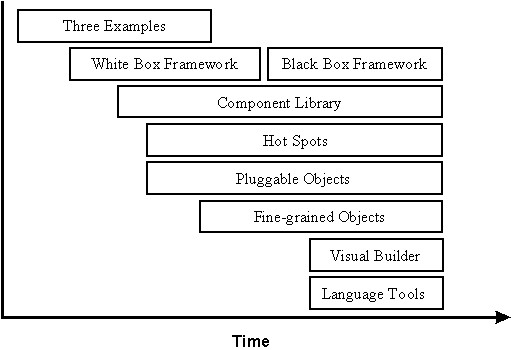
\includegraphics[width=.9\linewidth]{./obrazky-figures/evolving-frameworks.jpg}
\caption{The timeline of patterns as described in Evolving Patterns}
\end{figure}

To briefly describe the terms and how they relate to this work:
\begin{itemize}
\item \textbf{``Three Examples''} are three applications from which the framework will
draw common themes and architecture, so that it fulfills real-world needs. This
is what we will go through in the next section, where we take three existing
application specifications and build a Haskell version of it.
\item In a \textbf{``White Box Framework''}, the architecture is extracted into a separate
library and expanded or re-implemented in further applications. The author
emphasizes 'programming-by-difference', where the programmer extends library
code and later factors out commonly repeated patterns into the library. In
this work, this is the approach taken after implementing the ``Three Examples''
to create the basics of the shared libraries.
\item The next patterns, ``\textbf{Component Library}'', ``\textbf{Hot Spots}'', and
``\textbf{Pluggable/Fine-grained Objects}'' are all an extension of the above, focusing
on extracting concrete components and restructuring the architecture to
improve developer experience in specific ways. This level, nor the further
ones are not implemented in this work.
\item Skipping a ``\textbf{Visual Builder}'', which is not a common pattern in Web frameworks,
there are some basic ``\textbf{Language Tools}'' implemented as a part of creating the
libraries, namely a debugging console for watching specific values and an
inspector of the application storage. [TODO: specify after implementing]
\end{itemize}

Not mentioned as a part of the patterns but also an essential part of framework
development is thorough documentation and guides, as well as test coverage of
library code, which is also done as a part of the work on libraries in the
latter parts of this work.

The above is a quite general description, so we will now enumerate the specifics of the
implementation plan, starting with a reiteration of the requirements of a PWA
from the introduction, which is the end goal of this work.

\begin{itemize}
\item Pages are responsive on tablets \& mobile devices
\item All app URLs load while offline
\item Metadata provided for Add to Home screen
\item Page transitions do not feel like they block on the network
\item Each page has a URL
\item Pages use the History API
\item Site uses cache-first networking
\item Site appropriately informs the user when they are offline
\item Push notifications (consists of several related requirements)
\end{itemize}

There are, however, several components missing in the Haskell ecosystem that
need to be created from scratch:
\begin{itemize}
\item A full-featured browser routing library. While there are some existing
implementations, they are either incomplete or long abandoned.
\item A wrapper around ServiceWorkers
\item A push notifications library. This will need to be both a server-side library,
for creating them, and a client-side consumer, to parse them.
\item A way to prerender the application - either just the HTML ``app shell'' or all
pages on the site.
\item An offline storage library for the client. Here are several possible variants,
in the order of difficulty:
\begin{itemize}
\item plain storage datatype with LocalStorage, SessionStorage, and IndexedDB backends
\item a storage including a transparent cache integrated with the network layer
\item a storage with an invalidation or auto-refresh functionality, using an event
stream from the server
\item a storage with offline-capable synchronization capabilities
\end{itemize}
\end{itemize}

These components do not comprise a fully integrated framework in the sense of
e.g. Angular, such frameworks are quite uncommon in the Haskell ecosystem. More
common are collections of libraries that play well together, where one library
provides the fundamental datatype - the ``architecture'' of the application - and
other libraries fill in the functionality, which is what we will work on. Of the
proposed components, only the routing library is an ``architectural'' one in the
sense that it will influence the shape of the application and its fundamental
data types.

\section{Routing}
\label{sec:orgec8dadc}
A router is one of the basic components of a modern web application. There are
several features a router is concerned with: parsing the initial URL on
application start-up, changing it according to user navigation actions, storing
the navigation state for the rest of the application. In types, this might be
expressed as follows:

\begin{minted}[]{haskell}
parseRoute :: URL -> Route app
dispatchRoute :: Route app -> m ()
renderRoute :: Route app -> URL
\end{minted}

\subsection{Previous work}
\label{sec:org25b0dbf}
There are several widely used options for a server-side router, which has the
same responsibilities as a client-side one, and a very similar interface, for
the most part. These options differ in several ways, the most fundamental one
being the representation of the route, which in turns defines the basis of the
client API.

We will go through the routers of Yesod, Happstack, and Snap, all of them
popular Haskell frameworks for server-rendered web applications, and then move
on to Servant, a general-purpose routing solution for web services.

Yesod uses a special DSL (Domain Specific Language) for its router, which is
implemented via quasi-quoting, a specific flavor of meta-programming where an
arbitrary string is parsed into a Haskell expression. In this way Yesod
generates several type-class instances, implementations of the above-mentioned
functions, and a sum type containing all possible routes in an application. The
route itself is then just a plain data constructor of this sum type.

Happstack and Snap both offer a choice between using non-typed routes based on
strings, or type-safe routes similar to Yesod's approach above. For type-safe
routing, they both use the same library, \texttt{web-routes}. To use this library, the
user defines a sum type containing all possible routes in an application and
then uses library combinators to define a parser/encoder manually. The
parser/encoder is represented as a so-called \emph{boomerang}, a composable object
containing both directions of the transformation.

Servant is newer than the above options, and it is the most popular solution for
creating web APIs in Haskell at the moment. In Servant, an API is described
using a single large type in its entirety, created by composition using
type-level operators (\texttt{:<|>}, \texttt{:>}). This type is then processed using type-classes
to create specific types suitable for implementing a server or for creating
type-safe links. This type can also be interpreted using other libraries to
generate API documentation or clients in a variety of libraries.

Of these options, Servant's approach seems to be the most flexible one as is
also demonstrated by the large number of libraries that build on the Servant
core, although the complexity of using type operators and type interpreters may
be intimidating to developers looking beneath the user-facing API, at least
compared to the simplicity of the other two approaches which use plain functions
and simple sum types at their core.

TODO: Yesod, Web-routes, Servant-generic examples

\subsection{Servant}
\label{sec:org6be5c5b}
Servant is a general type-level DSL (Domain-Specific Language) in the domain of
web routing. An API defined using Servant is merely a type, a tree of type-level
terms composed using type operators. This API type is then interpreted using
type-level functions into value-level functions, e.g. routers.

\begin{listing}[htbp]
\begin{minted}[]{haskell}
type GetUsers = "users" :> QueryParam "sortby" SortBy :> Get '[JSON] [User]
type CreateUser = "users" :> ReqBody '[JSON] User :> Post '[JSON] UserId

data QueryParam (name :: Symbol) (a :: Type)

type UserAPI = GetUsers :<|>CreateUser

server :: Server UserAPI
server = (\sortBy -> return [users]) :<|> (\user -> saveUser user)

getUsers :: SortBy -> ClientM [User]
getUsers = f
  where
    (f :<|> _) = client (Proxy @UserAPI)
\end{minted}
\caption{Servant API definition:servant-api}
\end{listing}

A single Servant endpoint is shown in \ref{servant-api}. It is a composition of
symbols (type-level strings) and so-called \emph{combinators} like \texttt{QueryParam} and \texttt{Get},
which are usually defined as data types without any constructors as shown in the
second part of the snippet. These endpoints are then composed together using a
type-level alternation (``or'') operator, \texttt{:<|>}, as shown in the third part of the
snippet.

A server implementing such an API is defined in a very similar way, the handlers
for individual endpoints are composed together using the value-level operator
\texttt{:<|>}, as can be seen in the middle of the snippet. A client for the API is not
created by composition but by decomposition of the \texttt{:<|>} constructor as shown in
the last part of the snippet.

\begin{listing}[htbp]
\begin{minted}[]{haskell}
data UserAPI = UserAPI
  { _getUsers :: "users" :> QueryParam "sortby" SortBy :> Get '[JSON] [User]
  , _createUser :: "users" :> ReqBody '[JSON] User :> Post '[JSON] UserId
  } deriving (Generic)

server :: Server (ToServant UserAPI)
server = toServant $ UserAPI
  { _getUsers = \sortBy -> return [users]
  , _createUser = \user -> saveUser user
  }

getUsers :: SortBy -> ClientM [User]
getUsers = _getUsers apiClient
  where
    apiClient = genericClient @UserAPI
\end{minted}
\caption{Servant Generic API definition:servant-generic-api}
\end{listing}

An alternative approach to defining an API is using records. This approach uses
Haskell's support for datatype-generic programming to convert between a record
and a tree that uses \texttt{:<|>} on both the type-level and value-level. It is easier
to work with larger APIs in this way and it makes for easier-to-read type
errors. It is also possible to refer to individual endpoints using record
accessors, instead of (de)composition of the entire server or client. The code
in \ref{servant-generic-api} is functionally equivalent to the previous snippet,

The interpretation of an API type is done via type classes, a language feature
that is commonly compared to interfaces in object-oriented languages, but in
this case its use is a bit more involved. The API type is interpreted
recursively from the top, one combinator at a time starting from the outermost
\texttt{:<|>}. In the case of a server, the API type is also translated into the type of
the handler using an associated type family. Despite its name, a type family
defines a type-level function - given a type of an endpoint, find the type of a
handler.

We will see this process in more detail in a later section, when defining an
entirely new interpretation of an API type in the creation of a client router,
and when extending an existing interpretation to support prerendering of
applications on the server.

\subsection{Reflex}
\label{sec:orgf216372}
Before we dive into the implementation of the router, we also need to go through
the basics of Reflex, as its philosophy and building blocks constrain the
shape of any function we design.

As mentioned in the introductory sections, Reflex is a general \emph{Functional
Reactive Programming} (FRP) library.

FRP in general is a way of programming where the program consists of a network
of time-varying values and functions combining such values.

\begin{itemize}
\item TODO: More FRP intro
\end{itemize}

The basic building blocks of FRP are events, objects which have a value only on
a specific moment, and behaviors, which have a value at any point. Reflex adds
a third primitive, a \emph{dynamic}, which is a pair of a behavior and an event which
fires whenever the behavior changes.

Reflex is a general FRP library, to interact with the external world it needs
bindings to read external values and translate Reflex events into external
actions. There are several such bindings: \texttt{reflex-dom} for the browser,
\texttt{reflex-backend-wai} for the WAI web server interface, \texttt{diagrams-reflex} for SVG
animations, and several others. The one we will use in the rest of this work is
\texttt{reflex-dom}, which contains the necessary building blocks for web applications -
functions to create and animate HTML elements, listen on browser events, or
perform HTTP requests.

Reflex and Reflex-DOM provide the basic building blocks for creating
applications, but they don't fall to a natural structure for bigger applications
the way object-oriented frameworks do as in MVC and its variations. In fact, one
of the most common complaints of developers exploring Reflex is the lack of a
developed application architecture.

It is possible to recreate the Elm architecture in Reflex, as well as more
fine-grained architectures using small stateful components communicating with
top-level application logic. Several patterns have emerged so far, but none has
been generally accepted so far, and the one that has (Gonimo architecture, [TODO
ref]) requires a large amount of trivial ``plumbing'' code.

There are however several smaller structural patterns that have slowly emerged
as 'rules of thumb'. ``Dynamics as component inputs, events as outputs'' is one
such, which has been somewhat formalized as a combination of monad transformers
(\texttt{ReaderT} and \texttt{EventWriterT}) in Reflex itself.

Reflex is composed of several fine-grained typeclasses. These are abstract, and
they are translated into a series of monad transformers and their interpreters
on the top level.

There are several common methods of formalizing application architecture in
Haskell. Each method tries to abstract implementation details from application
logic by identifying all side-effects that a program requires and decomposing
them into individual effects. The methods are:

\begin{itemize}
\item Monad transformers and MTL-like typeclasses
\item ReaderT with a top-level application state
\item Effect interpreters (free monads, freer monads)
\end{itemize}

Each one has its advantages and disadvantages, and while they can be mostly
arbitrarily intermixed, each application or library usually chooses one. The
most popular in the Haskell community and used by the majority of libraries is
monad transformers and MTL-like classes, which is also the method that Reflex
uses.

A signature of a component in a program structured in this way would look
something like \ref{mtl-api}, where first two constraints of \texttt{userView} would be
executed using the function \texttt{runApp}, with the remaining \texttt{MonadWidget} being
executed by the top-level rendering function.

\begin{listing}[htbp]
\begin{minted}[]{haskell}
userView ::
     (MonadReader AppState m, MonadRouter AppRoute m, MonadWidget t m)
  => Dynamic t User
  -> m (Event t UserEdit)

runAppM :: MonadWidget t m => RouterT AppRoute (ReaderT AppState m) a -> m a
\end{minted}
\caption{MTL-based API:mtl-api}
\end{listing}

\subsection{Implementation}
\label{sec:org59b5d42}

I have decided to use Servant's approach in my work, as it seems to be the most
flexible and extendable one.

My contributions in this area are:
\begin{itemize}
\item a client-side router using Reflex's FRP types
\item an extension of the server-side router to support rendering Reflex applications
\item a static site generator
\item JAM-stack-like web
\item a combinator to more easily work with servant-generic types (\texttt{.>})
\end{itemize}

TODO: demonstrate client router approach (a few type class instances and the
top-level router)
TODO: demonstrate in-app links
TODO: demonstrate App instance of HasServer

\subsection{Possible extensions}
\label{sec:orgbea0c44}
Next work:
\begin{itemize}
\item AuthProtect, AuthRoleProtect
\item route matcher for route checks (separate typeclass)
\end{itemize}

\section{Service workers}
\label{sec:orgddac874}
TODO: general intro

\subsection{Requirements}
\label{sec:org8c06d49}
The Service Worker features that we aim to support are: precaching, fetch
control, and push notifications.

Precaching means storing the files essential for the application into cache as
soon as the Service Worker starts. This way, the application is able to run
offline. These files usually include \texttt{index.html}, the application entrypoint;
\texttt{bundle.js} (or similar), the JavaScript bundle containing the entire application,
and \texttt{bundle.css}, a bundle with all application styles. Application icons and
fonts are usually included as well, as are analytics libraries for usage
tracking.

Fetch control in this context means intercepting all outgoing requests from the
application, and deciding what to do with them based on the URL or method. This
feature has many use-cases, e.g. using the precached application files when
offline, checking for a new version of the application and notifying the user;
storing external fetched resources into cache to save data, or storing outgoing
analytics requests into a queue when offline and only sending them when the user
later connects to the Internet.

Push notifications are the feature for which service workers are most well
known. They allow a web application to send notifications to any of its clients,
where the application can choose to arbitrarily process the notification.

The basis of the implementation is a single dependently typed record that
contains the entire configuration of the worker. This record is then used in
three different contexts: to generate the worker JavaScript and serve it over
HTTP, in the client for any interactions with the worker (e.g. to subscribe to
push notifications), and on the server for sending the notifications, as
illustrated by \ref{service-worker-api}.

\begin{listing}[htbp]
\begin{minted}[]{haskell}
generateWorker :: ServiceWorker push -> ByteString
runServiceWorkerClientT :: ServiceWorker push -> ServiceWorkerClientT push m a -> m a
runPushServerT :: ServiceWorker push -> PushT push m a -> m a
\end{minted}
\caption{Service Worker API:service-worker-api}
\end{listing}

While I'd originally intended to create the service worker using GHCJS and the
JavaScript FFI (Foreign Function Interface), there is an obstacle that prevents
that: service workers do not run in the same way that a regular browser
application does. A browser can terminate a service worker at any time to save
computing resources, and restarts it when it is needed to process application
events, so a service worker is expected to contain mostly just event handlers.

This is however at odds with the GHCJS execution model which relies on
\texttt{setTimeout} or \texttt{requestAnimationFrame} to support multiple threads, asynchronous
execution, and other features needed to run the entirety of Haskell in the
browser. That means that we cannot use GHCJS to create Service Workers and need
to generate plain JavaScript code instead.

\subsection{JMacro}
\label{sec:org6ebfda8}
Of the options available for generation of JavaScript in Haskell, only the
library JMacro is suitable for this task, as it is the only library intended for
this purpose, none of the other libraries are very user-friendly.

JMacro allows the user to write plain JavaScript code embedded in Haskell via
quasi-quotation, which is a method of meta-programming that makes it possible to
transform arbitrary strings into Haskell expressions. The library supports the
entirety of ECMAScript 3, so most existing JavaScript code can be copy-pasted
without the need for changes, as long as it doesn't use the features of newer
ECMAScript versions. JMacro is untyped, it recognizes two forms of JavaScript
code, expressions and statements. It also supports injection of Haskell
variables using anti-quotation. An example of JMacro code can be seen in \ref{jmacro}.

\begin{listing}[htbp]
\begin{minted}[]{haskell}
handleFetch :: JExpr -> JStat
handleFetch fn = [jmacro|self.addEventListener('fetch', `(fn)`);|]

sw :: JStat
sw = handleFetch [jmacroE|
function(evt) {
  console.log('The service worker is serving the asset.');
  evt.respondWith(fromNetwork(evt.request, 400).then(null, function () {
    return fromCache(`(cacheName)`, evt.request);
  }));
}|]
\end{minted}
\caption{An example of JMacro:jmacro}
\end{listing}

\subsection{Implementation}
\label{sec:org83f89fe}
The three features of service workers that we want to support (prefetch, fetch
control, push notifications)

Prefetch is simple, only save the requested files into cache in the onInstall
handler.

Fetch is a bit more involved. In the onFetch handler, we need to find out if the
outgoing request matches any of the configured filters, so we go through the
filters in order and if a request matches, the selected cache strategy is
executed. There are many possible behaviors with regards to caching and network
access. We cannot cover all possible cases, but we can cover common ones. These
are encoded as a plain sum type, which can be seen in \ref{cache-strategy}. Most
strategy names are self-explanatory, I will mention only \texttt{StaleWhileRevalidate}
and its \texttt{Notify} variation: these serve the currently cached version of a
resource, and attempt to fetch a newer one, which will then be stored into cache
for later requests. This strategy is often used for main application files,
which is the reason for the \texttt{Notify} variation, which will also notify the
application itself if there is a newer version available and the application can
then notify the user.

\begin{listing}[htbp]
\begin{minted}[]{haskell}
data CacheStrategy
  = CacheFirst Text
  | CacheOnly Text
  | NetworkFirst Text
  | NetworkOnly
  | StaleWhileRevalidate Text
  | StaleWhileRevalidateNotify Text
  deriving (Eq, Ord, Show)
\end{minted}
\caption{Cache strategies:cache-strategy}
\end{listing}

TODO: Talk about matchers

Handling push notifications is not trivial either. While using them in the most
basic way is as simple as calling \texttt{showNotification} on the body of the incoming
message, it is possible to do more, like passing the notification to the
application using \texttt{postMessage}. Like with cache strategies, it is not possible to
cover all possible use-cases with predefined options so again, we add the common
ones. This time, they need to be encoded as a \emph{GADT} (Generic Algebraic Data Type),
an extension of Haskell data types that allows us to specialize the type of a data
constructor, which we can use to specialize the types of sending and receiving
functions in client and server code.

The options I have selected for the library are included in
\ref{push-behaviors}. \texttt{Ignore} has the type \texttt{Void} as its parameter, which is an empty
type that can have no valid values (excluding \texttt{undefined}), which means that it is
impossible to call a sending function in server code. \texttt{Ignore} has no handler code
generated in the service worker. \texttt{ViewOnly} displays a notification without any
further handling. \texttt{ViewAndOpen} and \texttt{ViewAndProcess} both add another event handler
that listens for the user clicking on the notification, which will open the
application if closed, and switch to the application window if open but not
focused. \texttt{ViewAndProcess} and \texttt{ProcessOnly} will also pass the message to the
application for further processing via \texttt{postMessage}.

\begin{listing}[htbp]
\begin{minted}[]{haskell}
data PushBehavior a where
  PushIgnore :: PushConfig Void
  PushViewOnly :: PushConfig ()
  PushViewAndOpen :: PushConfig ()
  PushViewAndProcess :: FromJSON a => PushConfig a
  PushProcessOnly :: FromJSON a => PushConfig a
\end{minted}
\caption{Push behaviors:push-behaviors}
\end{listing}

The rest of the service worker generation does not contain any non-obvious code,
so I will skip it. It is included with the rest of the source code on the
attached data storage.

The server part of this component is made up of two parts: generating and
serving the service worker code, and sending push notifications.

Serving the service worker is done by creating a new instance of the method
\texttt{MimeRender,} which tells the server how to render a value to a binary format.

The ability to send push notifications is added to handler code using a monad
transformer and a type class containing a single method, \texttt{sendPushNotification}.
The monad transformer contains a ReaderT containing the server VAPID keys, which
are necessary for\ldots{} This transformer uses Servant ``context''
capabilities\ldots{} TODO: finish this.

TODO: describe client class methods (mainly for the dependent types + interpreter)

\subsection{Possible extensions}
\label{sec:org98a9962}
The obvious follow-up work is supporting more features of service workers:
fine-grained cache control with resource expiration based on its age or available
storage space; or \emph{Background Sync}, an API for queuing requests mane when the device
was offline to be retried whenever it goes online, whether the application is
open or closed.

Supporting more exotic use-cases is also possible next work, use-cases like
communication between multiple instances of an application using the service
worker as a relay, or using fetch control as a load balancer to dynamically
switch between servers from which the application downloads data.

However, there is another approach that would obsolete most of the work on this
component: after creating this component, I have discovered a project trying to
create a typed DSL (Domain-Specific Language) for generating JavaScript, \texttt{jshark}
(TODO: ref). While I originally disregarded the approach of making a typed DSL
instead of a library with a fixed selection of options, as the DSL would need to
be able to represent arbitrary JavaScript logic, using this library (or a
similar one) would allow building a hierarchy of functions hiding more and more
of the underlying logic. However, as of the time of writing, this library is
still unfinished, so writing a service worker builder using a typed DSL stays a
project for the future.

A hypothetical example of such approach can be seen in
\ref{jshark}, which demonstrates more complex usage of fetch control, dispatching
requests based on their destination (the originator of a request, e.g. \texttt{"style"}
corresponds to a \texttt{<style>} tag or a CSS include).

\begin{listing}[htbp]
\begin{minted}[]{haskell}
sw :: WorkerM ()
sw = self `on` fetch $ \event -> do
  dest <- event ^. request . destination
  switch dest $ do
    case_ "font" $
      respondWith event cacheOnly
    cases_ ["style", "script", "document", "image"] $
      respondWith event networkFirst
    default_ $
      respondWith event networkOnly
\end{minted}
\caption{Service worker using a JavaScript DSL:jshark}
\end{listing}

This approach may also be combined with code generation from WebIDL, an
interface definition language for the Web (TODO: ref) used e.g. in the Chromium
browser, to produce an API that exactly corresponds to the underlying JavaScript
one, only with strong types. Generating an API from WebIDL has a precedent in
the library \texttt{ghcjs-dom}, a library that provides a strongly-typed interface to
most browser APIs, which generates most of its code in this way.

\section{Storage}
\label{sec:org9b455bb}
A storage library can be implemented in many ways.

TODO: describe possible options, all the way to PouchDB and Datascript

In this regard, I am not looking to build a library with many features but
merely a building block that can serve basic purposes. The goal of this section
is to build an in-memory key-value store synchronized with the LocalStorage
browser API. The API of the store interface is simple, as shown by
\ref{storage-api}, but it can serve not only as a simple cache, but also as a way
to prerender data into HTML directly on the server, which would also enable
using Reflex as a static site generator.

\begin{listing}[htbp]
\begin{minted}[]{haskell}
get :: Behavior t (Key e) -> m (Dynamic t (Maybe e))
getAll :: m (Dynamic t (Map (Key e) e))
put :: Event t (Key e, Maybe e) -> m ()
\end{minted}
\caption{Storage API:storage-api}
\end{listing}

There are several ways of extending the API like adding expiration (automatic
or manual) so that it can better serve as a cache (e.g. function \texttt{getOrFetch}),
but this is sufficient for many use-cases.

TODO: Refer to the \ref{sec:orgf216372} section

\chapter{Developing an application}
\label{sec:org4b90b44}
The components we created above enable a variety of use-cases:
\begin{itemize}
\item compiling an interactive browser application into a small bundle
\item creating a Progressive Web Application and prerendering it on the server, so
that it is usable even in browsers with JavaScript disabled
\item generating a static site using data from external sources (e.g. a database)
\item combining the above to create a site with full-stack interactive
administration that generates a static public site
\end{itemize}

TODO: Correct if I don't manage 'Blog'

In this section, we will go through the tasks common to all of these use-cases
and in the next one, we will look at the specifics of creating each one.

\section{Development tools}
\label{sec:orge0a597c}
The basis of Reflex's development platform is Nix, development environment is
nix-shell.

An editor common in the Haskell world is Emacs, and most documentation on
setting up an editor for frontend development is in fact aimed at Emacs. Other
editors are also supported, but there is usually no or little documentation.

A tool that greatly eases setting up development environment is direnv, which is
able to load 

TODO: Nix, editor integration, development process
TODO: Prelude, code structure
TODO: Describe component development in detail
TODO: Authorization
TODO: Tests
TODO: Common tasks in webdev - defining entities, migrations, audit logs, defining the API
TODO: Deployment

\section{Deploy}
\label{sec:orge451aa2}
\begin{itemize}
\item static only = bundled executable
\item executable + assets separately
\item Nix, Keter, standalone, Ansible for deployment - interoperability with classical DevOps
\end{itemize}

\subsection{Nix}
\label{sec:orga63bd9b}
\begin{listing}[htbp]
\begin{minted}[,frame=single]{nix}
{ stdenv, fetchurl, perl }:

stdenv.mkDerivation {
  name = "hello-2.1.1";
  builder = ./builder.sh;
  src = fetchurl {
    url = ftp://ftp.nluug.nl/pub/gnu/hello/hello-2.1.1.tar.gz;
    sha256 = "1md7jsfd8pa45z73bz1kszpp01yw6x5ljkjk2hx7wl800any6465";
  };
  inherit perl;
}
\end{minted}
\caption{An example Nix derivation of GNU hello}
\end{listing}

One technology not yet mentioned, but upon which will stand the entire build
system used in this work from compiling to deploying, is Nix. Nix
\cite{dolstra2006purely} is a package manager with focus on reproducibility and
isolation, described as a 'purely functional package manager' - every package is
built in isolation by a 'pure function' without side-effects, and the result is
immutable. When installing a package packaged in such a way, the exact versions
of dependencies are installed and used as well (identified by a SHA-256 hash) -
all runtime dependencies all the way up to \texttt{libc}.

Nix is a declarative build tool and a package manager, similar in purpose to
Make and in philosophy to Haskell. There are other tools built on top of Nix
though, the most interesting being NixOS, a declarative operating system, and
NixOps, a cloud deployment tool \cite{dolstra2008nixos}. Nix shines at
cross-compilation, which is the main reason we will use it in this work -
compiling to JavaScript or Android/iOS is trivial after the initial setup.

\chapter{Case studies}
\label{sec:orga9df510}
\begin{itemize}
\item brief descriptions of tasks
\item screenshots
\item code structure
\begin{itemize}
\item domain design
\item architecture
\item file structure
\end{itemize}
\item comparison with JS in general
\begin{itemize}
\item feature parity
\item ergonomics
\item CLOC
\end{itemize}
\end{itemize}

\section{Workflow and tools}
\label{sec:org8dd62d1}
\begin{itemize}
\item TODO: describe the development flow of an app built using these tools

\item editor tooling
\item application structure
\item QA (tests, e2e, CI, \ldots{}), documentation
\item development tool options
\item deployment options
\end{itemize}

\section{TodoMVC}
\label{sec:orge2f7193}
There is an abundance of web frameworks, and there are several projects that aim
to give developers a side-by-side comparison of them. Out of these, the original
and most well-known one is TodoMVC \cite{todomvc}, which is aimed at ``MV* frontend
frameworks''. There are currently 64 implementations of their specification -
some of them are variants of the same framework though. There are a few others -
HNPWA is aimed at Progressive Web Applications and it is a tad smaller, with 42
implementations. The last comparison project selected for this work is
RealWorld. This one has both a frontend and a backend part and there is also a
small number of full-stack frameworks. It offers a quite thorough comparison,
with 18 frontends, 34 backends, and 3 full-stack implementations.

We will start with TodoMVC as it is the simplest of the three. TodoMVC is, as
the name hints, a web application for managing a to-do list. It is not a complex
project but it is intended to exercise fundamental features of a framework - DOM
manipulation, forms and validation, state management (in-memory and in
LocalStorage), and routing.

\section{HNPWA}
\label{sec:org7662cf7}
-- demonstrate that it works without JavaScript!

HNPWA \cite{hnpwa} is a client for Hacker News, a technological news site. Unlike TodoMVC,
HNPWA does not provide a rigid specification and consists only of a rough
guideline of what to implement. The task is to create a Progressive Web
Application that displays information from a given API. The application must be
well optimized (to achieve score 90 in the Lighthouse tool) with optional
server-side rendering.

\section{RealWorld}
\label{sec:org89ab794}
RealWorld \cite{realworld} is the most complex of the comparison projects. It is a clone of
Medium, an online publishing platform, so it requires everything a ``real world''
application would. The task is split into a backend, defined by an API
specification, and a frontend, defined by an HTML structure.

There is a number of features the application needs to support, namely: JWT
(JSON Web Token) authentication with registration and user management, the
ability to post articles and comments, and to follow users and favorite articles.

\section{Blog}
\label{sec:org39dd976}
-- statically generated with a FRP admin interface

\chapter{Conclusion}
\label{sec:orga2dc283}
TODO: return to the comparison with JS, PHP, \ldots{} frameworks

\section{Follow up work}
\label{sec:org9b26072}
\begin{itemize}
\item extending the storage library capabilities, a Datascript-like query language,
bindings to more backends, leveraging IndexedDB capabilities
\item effects in Reflex, more flexible extension mechanism
\item CSS-in-Haskell (a la CSS-in-JS)
\item typed assets - TH to generate, then typed <img>, <link> components
\item router extensions - access gating (auth'd, per-role)
\item debugging tools to run inside the browser - variable watching, state inspecting
\item client crash reports
\item end-to-end testing tools (asserts on both back- and frontend?)
\item dynamic user-provided content - parsing a HTML alike, preregistered named
components, an editor
\item synchronization library
\item form library
\item GraphQL for interop with modern JS frameworks
\end{itemize}

\section{In closing}
\label{sec:org7d3e43d}
-- The final chapter includes an evaluation of the achieved results with a special
emphasis on the student's own contribution. A compulsory assessment of the
project's development will also be required, the student will present ideas
based on the experience with the project and will also show the connections to
the just completed projects. \cite{Pravidla}

% * (bibliography, start of appendix)                           :ignoreheading:
\makeatletter
\def\@openbib@code{\addcontentsline{toc}{chapter}{Bibliography}}
\makeatother
\bibliographystyle{bib-styles/englishiso}

\begin{flushleft}
\bibliography{projekt}
\end{flushleft}
\iftwoside\cleardoublepage\fi

% Appendices
\appendix
\appendixpage
\iftwoside\cleardoublepage\fi

\startcontents[chapters]
% \setlength{\parskip}{0pt}
% \printcontents[chapters]{l}{0}{\setcounter{tocdepth}{2}}
% \setlength{\parskip}{0.5\bigskipamount}
\iftwoside\cleardoublepage\fi

\chapter{Contents of the attached data storage}
\label{sec:orgc31e159}
TODO: fill in

\chapter{Poster}
\label{sec:org2e054ec}
TODO: fill in
\end{document}